% !TEX root = ../main.tex

\section{Bayesian Optimization}
\label{sec:opt:BO}
Bayesian optimization (BO, \cite{jones1998efficient,osborne2009gaussian,brochu2010tutorial,shahriari2016taking})  is a 
global optimization scheme that requires only that the target
function can be evaluated (noisily) at any given point.  It is derivative-free,
naturally incorporates noisy evaluations, and is typically highly efficient 
in the number of function evaluations.  It is therefore highly suited to
problems where the target function corresponds to the output of a simulator,
estimation scheme, algorithm performance evaluation, or other cases where
the target is not known in closed form.  It has been successfully applied to 
a number of applications \todo{ADD} and remains a fast growing area of
active research.

The key idea of BO is to place a prior on $f$ that expresses belief about the space of functions within which $f$ might live.  When the function is evaluated, the resultant information is incorporated by conditioning upon the observed data to give a posterior over functions.  
This allows estimation of the expected value and uncertainty in $f\left(\theta\right)$ for all $\theta \in \vartheta$.  
From this, an acquisition function $\zeta : \vartheta \rightarrow \real$ is defined, which assigns an expected utility to evaluating $f$ at particular $\theta$, based on the trade-off between exploration and exploitation in finding the maximum.  When direct evaluation of $f$ is expensive, the acquisition function constitutes a cheaper to evaluate substitute, which is optimized to ascertain the next point at which the target function should be evaluated in a sequential fashion.  By interleaving optimization of the acquisition function, evaluating $f$ at the suggested point, and updating the surrogate, BO forms a global optimization algorithm that is typically very efficient in the required number of function evaluations, whilst naturally dealing with noise in the outputs.  

Although alternatives such as random forests \citep{bergstra2011algorithms,hutter2011sequential} 
or neural networks \citep{snoek2015scalable} exist, the most common surrogate model used for 
$f$ is a Gaussian process (GP) \citep{rasmussen2006gaussian}.  Their are a number
of characteristics that make GPs suitable for the surrogate model.  For example, they are very powerful
regressors that can accurately represent the function from relatively few evaluations, especially
for low-dimensional smooth functions.  They also naturally produce uncertainty estimates
that are typically more accurate that those produced by alternatives \todo{Citation?} which often
have to resort to post-processing or heuristics to estimate uncertainty.
It also leads to simple and tractable acquisition functions.  Similarly, their ability to incorporate
noisy observations is be very convenient.  When prior information is known about the function, the
flexibility in choosing the covariance kernel can also be very helpful, for example allowing known
smoothness to be incorporated.  However, this can also be a curse as an inappropriate choice of
kernel can severely happen the performance.  In particular, it will typically be necessary to
do inference over, or at least optimize, the GP hyperparamters.  Another drawbacks to using GPs
is poor scaling in the number of iterations - training is a $O(N^3)$ operation due to the required
matrix inversion.  This typically restricts BO using GPs to using at most hundreds of iterations
unless appropriate approximations are made~\citep{snelson2006sparse,hensman2013gaussian}.
Another drawback can be poor scaling in the dimensionality of the inputs - most common kernels
rely on local modelling which can break down in high dimensions because points are typically
far away from one another \citep{bengio2006curse}.

\begin{figure}[t]
	\centering
	\begin{tabular}{m{0.65\textwidth} m{0.15\textwidth}}
	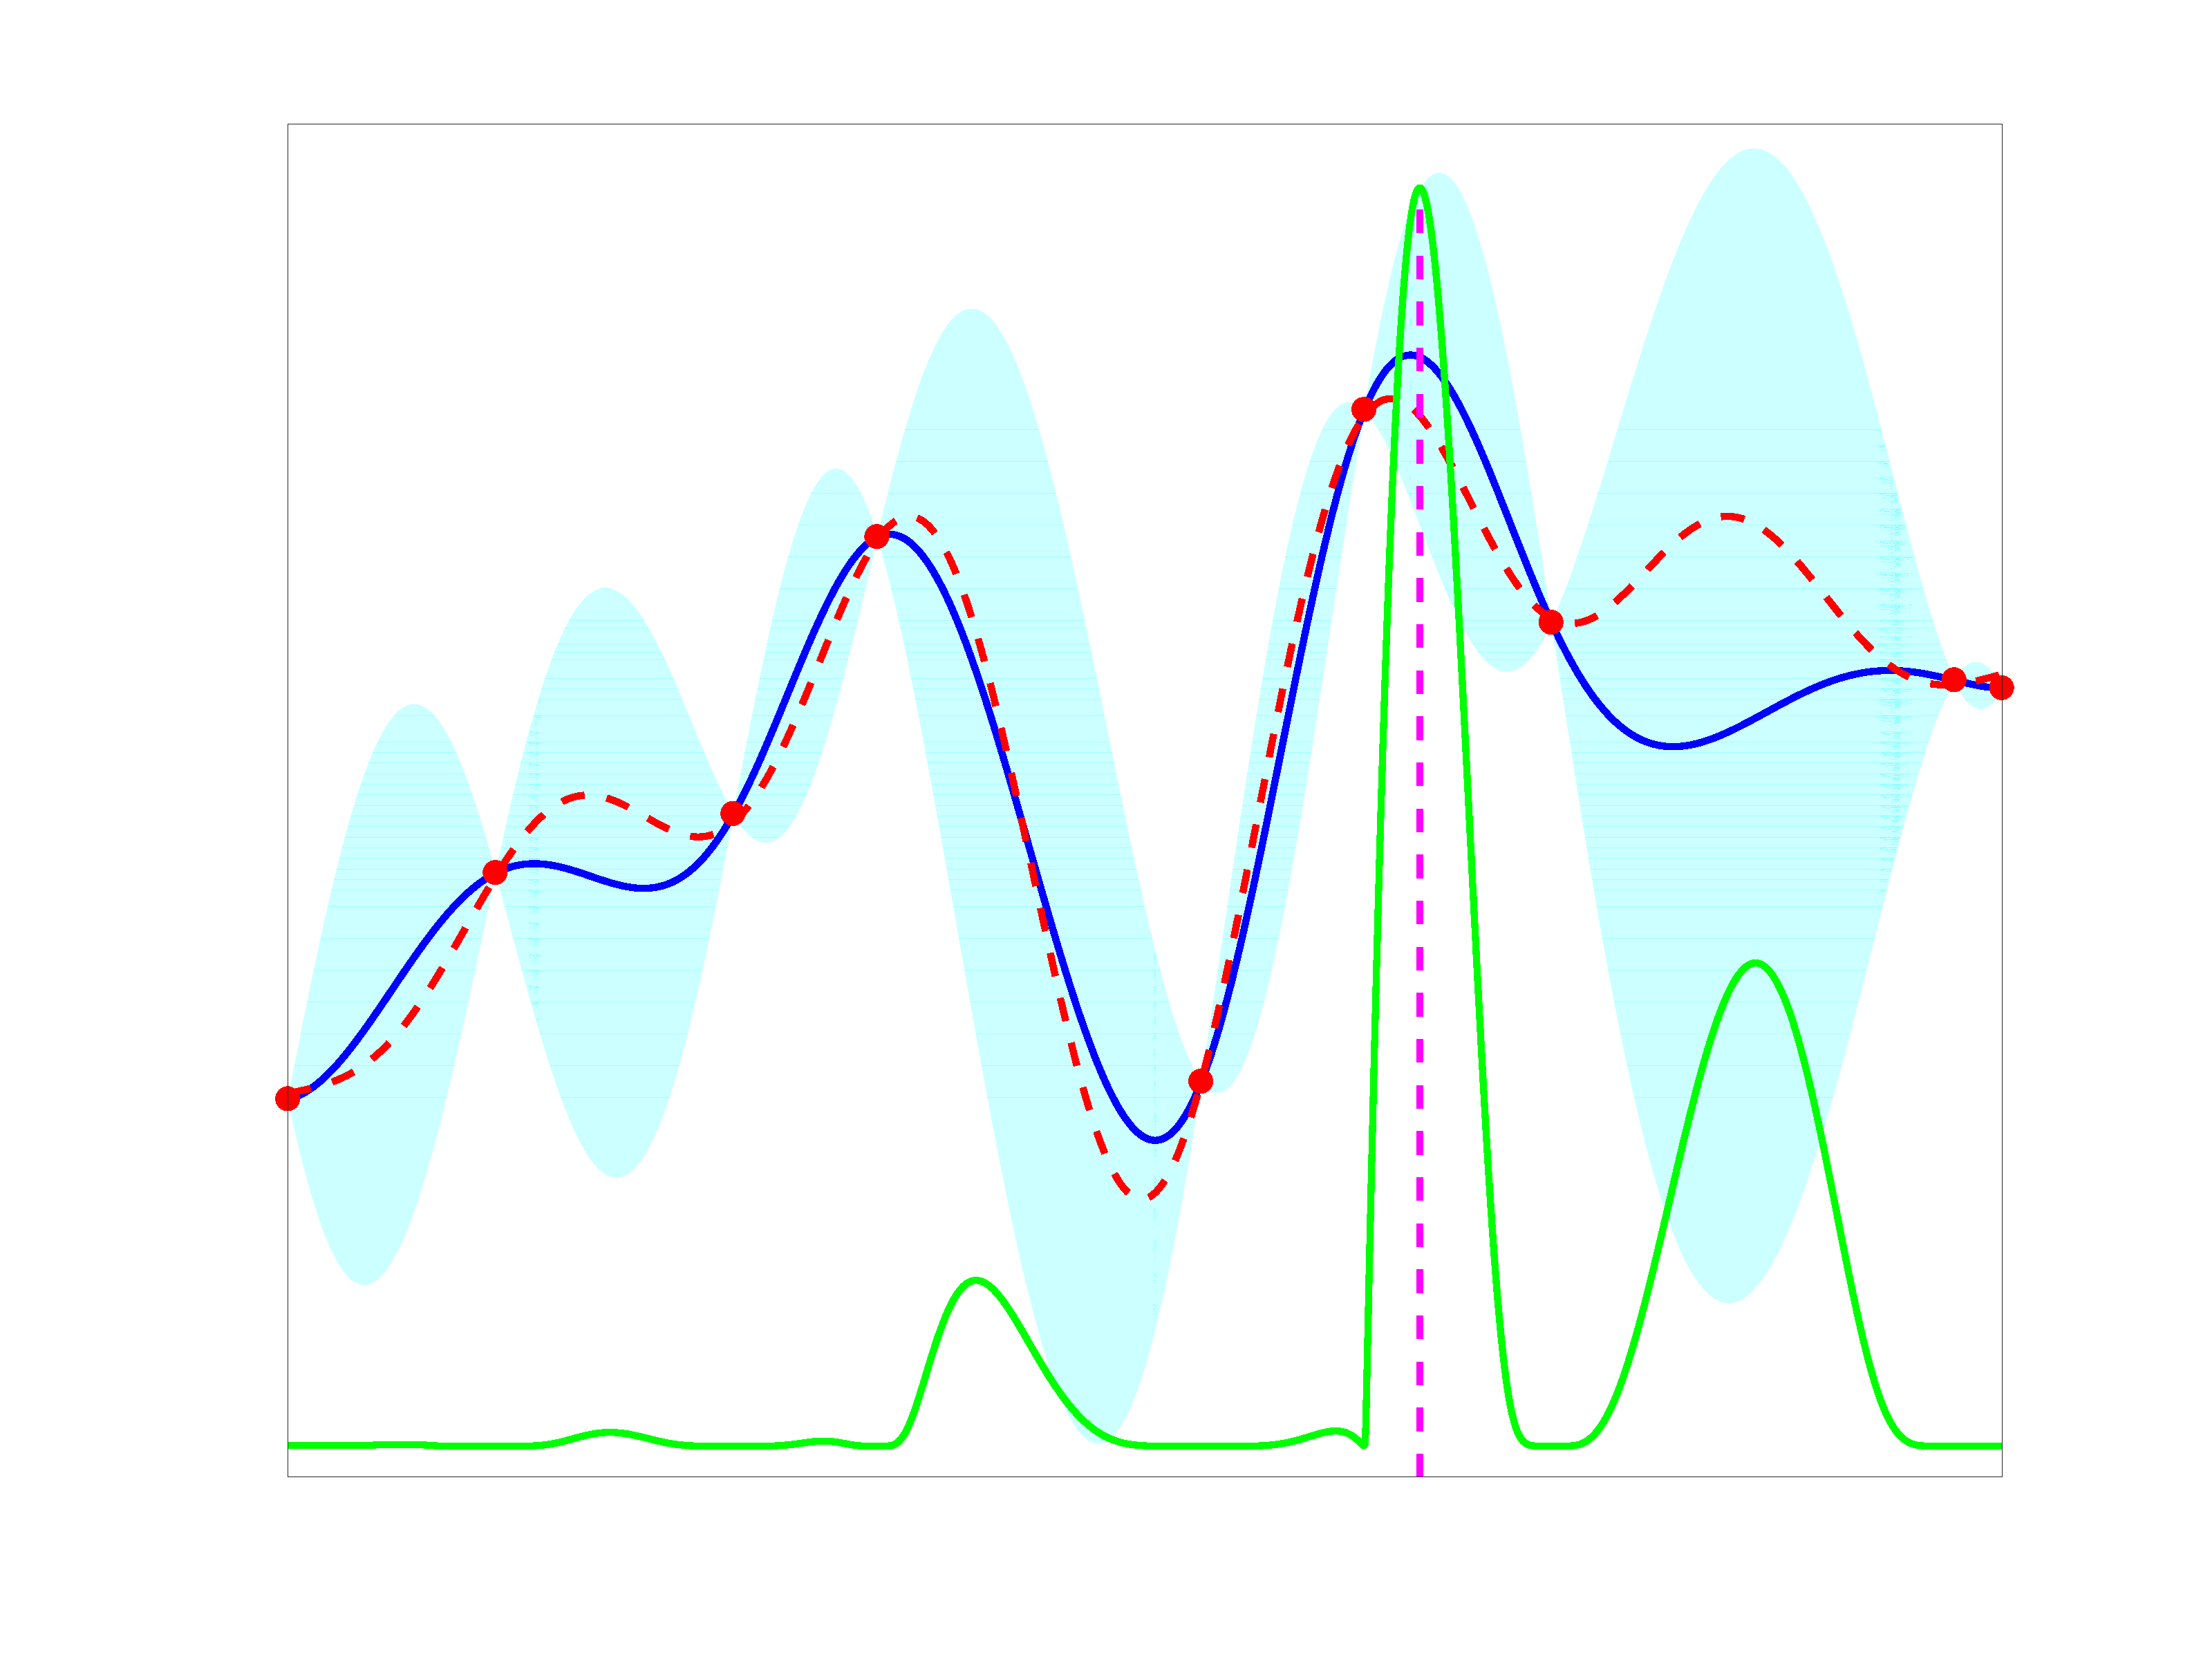
\includegraphics[width=0.6\textwidth]{10_with_acq_opt} & 10 Iterations
	\\
	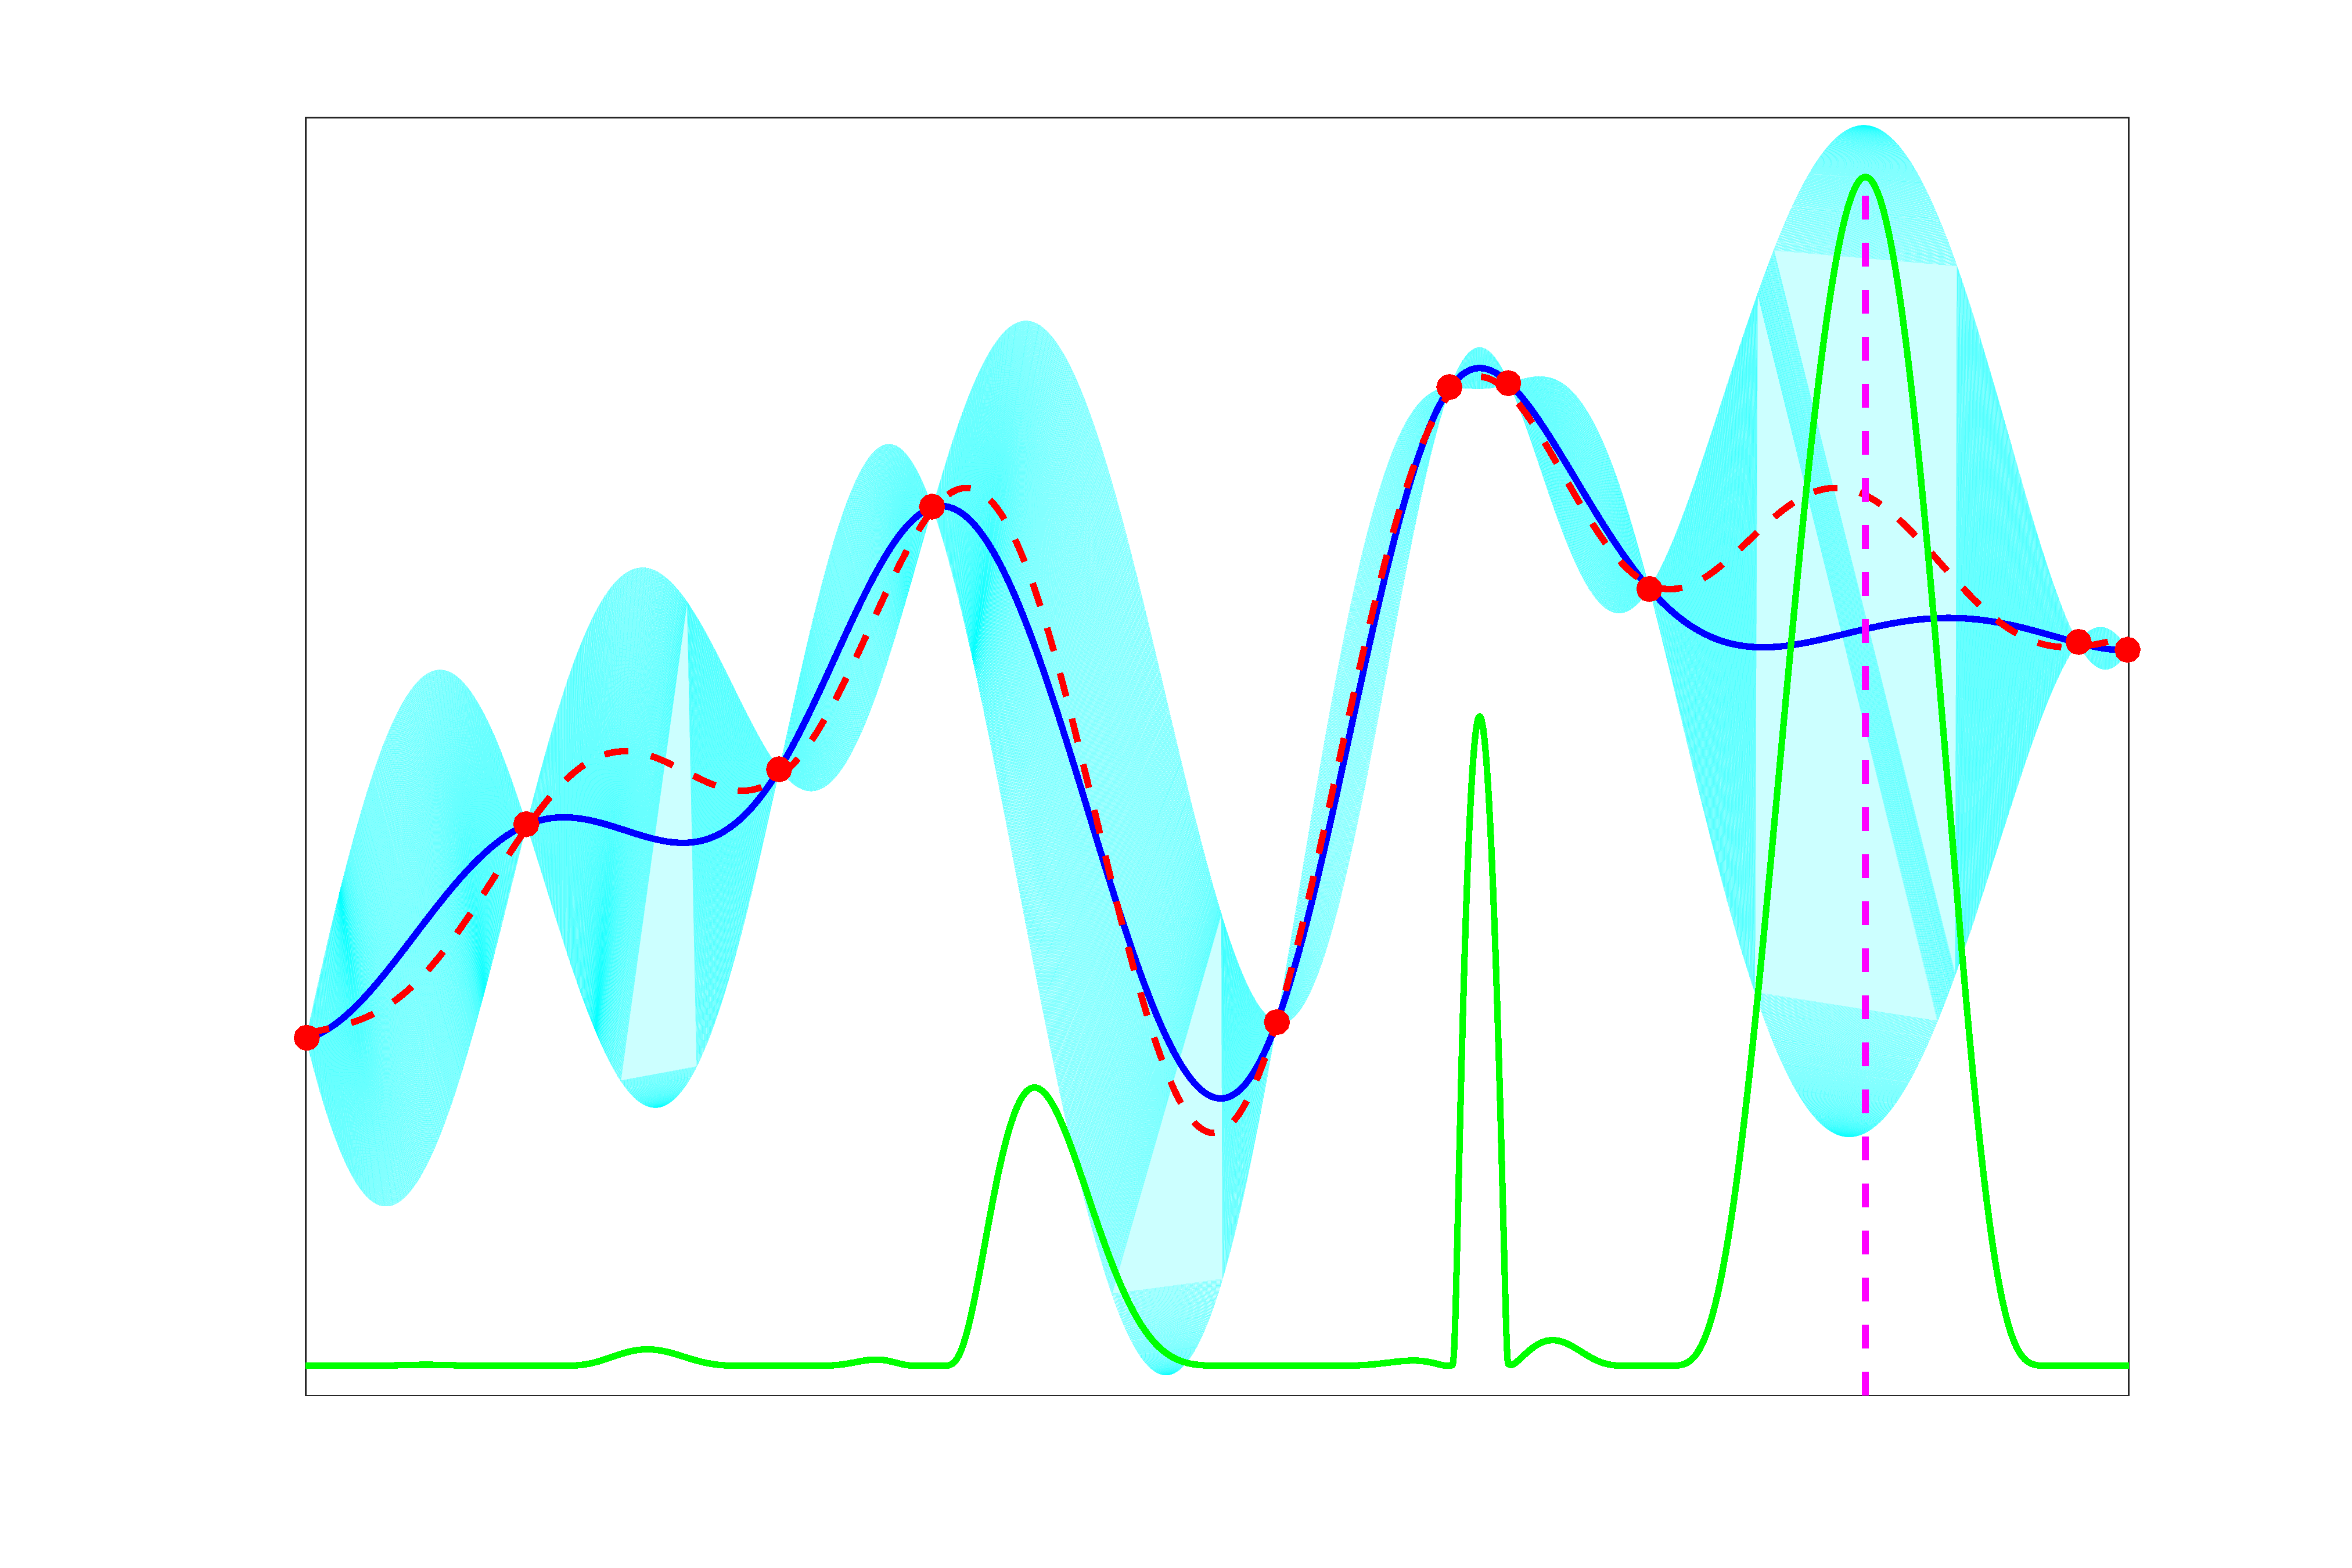
\includegraphics[width=0.6\textwidth]{11_with_acq_opt} & 11 Iterations
	\\
	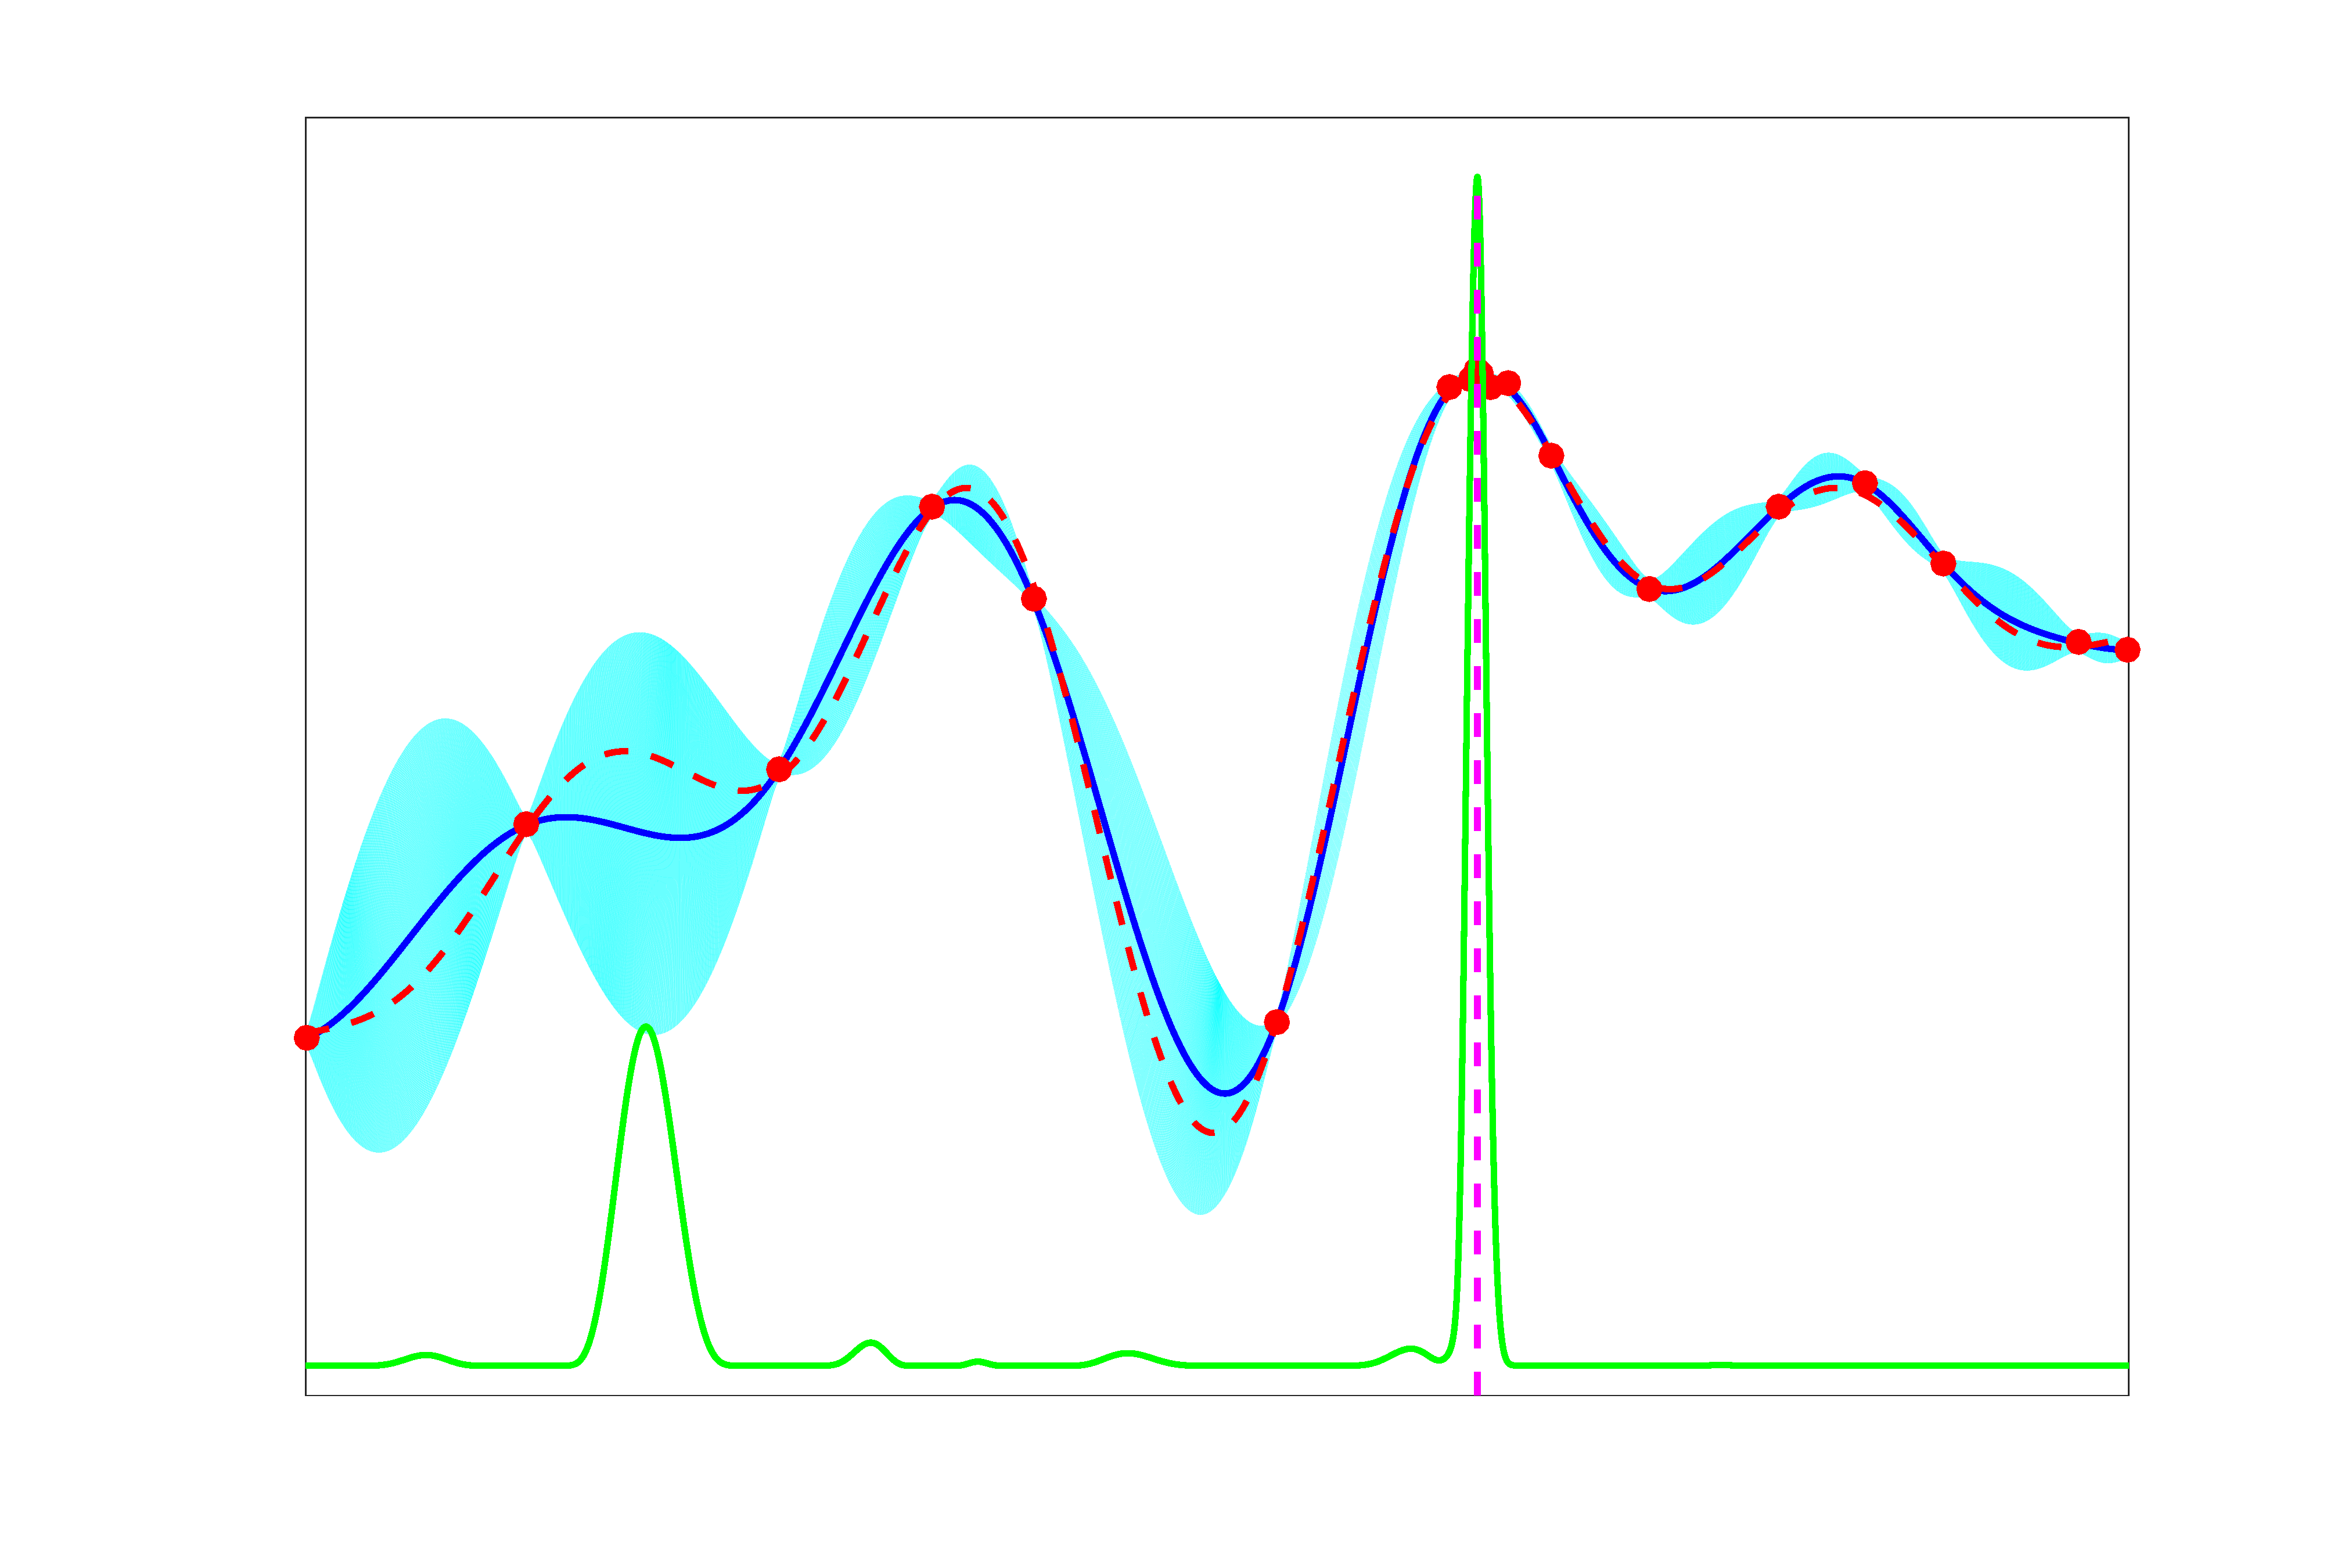
\includegraphics[width=0.6\textwidth]{20_with_acq_opt} & 20 iterations
	\end{tabular}
	\caption{Illustration of using Bayesian optimization method to optimize the
		toy one dimensional problem given in~\eqref{eq:opt:toy}.  Red dots show
		the function evaluations,  the dotted red line shows the true function, 
		the solid blue line is the GP mean, the shaded region is the GP mean $\pm 2$
		standard deviations, the green line is the acquisition function, and
		the dotted purple line is the location of the maximum of the acquisition
		function. \label{fig:opt:bayes-opt}}
\end{figure}

Figure~\ref{fig:opt:bayes-opt} provides a overview of the BO approach for optimizing the 
following simple one dimensional problem
\begin{align}
\label{eq:opt:toy}
f(\theta) = \frac{\theta}{15}-\frac{\theta^2}{50}-\frac{\sin \theta}{\theta}, \quad -5\le \theta \le 5
\end{align}
with noisy observations $v\sim\mathcal{N}(f(\theta),0.01^2)$.
